The previous chapter developed a mathematical relationship between the position of a point $P$ in a scene (expressed in world frame coordinates $P_W$), and the corresponding point $p$ in pixel coordinates that gets projected onto the image plane of the camera. This relationship was derived based on the pinhole camera model, and required knowledge about the camera's intrinsic and extrinsic parameters. Nonetheless, even in the case where all of these camera parameters are known it is still impossible to reconstruct the depth of $P$ with a single image (without additional information).
However, in the context of robotics, recovering 3D information about the structure of the robot's environment through computer vision is often a very important task (e.g. for obstacle avoidance). Two approaches for using cameras to gather 3D information are therefore presented in this chapter, namely \textit{stereo vision} and \textit{structure from motion}\cite{SiegwartNourbakhshEtAl2011}\cite{ForsythPonce2011}.


\notessection{Stereo Vision and Structure From Motion}
Recovering scene structure from images is extremely important for mobile robots to safely operate in their environment and successfully perform tasks. While a number of other sensors can also be used to recover 3D scene information, such as ultrasonic sensors or laser rangefinders, cameras capture a broad range of information that goes beyond depth sensing. Additionally, cameras are a well developed technology and can be an attractive option for robotics based on cost or size.

Unfortunately, unlike sensors that are specifically designed to measure depth like laser rangefinders, the camera's projection of 3D data onto a 2D image makes it impossible to gather some information from a single image\footnote{Unless you are willing to make some strong assumptions, for example that you know the physical dimensions of the objects in the environment.}. Techniques for extracting 3D scene information from 2D images have therefore been developed that leverage \textit{multiple} images of a scene. Examples of such techniques include \textit{depth-from-focus} (uses images with different focuses), \textit{stereo vision} (uses images from different viewpoints), or \textit{structure from motion} (uses images captured by a moving camera).


\subsection{Stereo Vision}
Stereopsis (from \textit{stereo} meaning solidity, and \textit{opsis} meaning vision or sight) is the process in visual perception leading to the sensation of depth from two slightly different projections of the world onto the retinas of the two eyes. The difference in the two retinal images is called horizontal \textit{disparity}, retinal disparity, or binocular disparity, and arise from the eyes' different positions in the head. It is the disparity that makes our brain fuse (perceive as a single image) the two retinal images, making us perceive the object as one solid object. For example, if you hold your finger vertically in front of you and alternate closing each eye you will see that the finger jumps from left to right. The distance between the left and right appearance of the finger is the disparity.

Computational stereopsis, or \textit{stereo vision}, is the process of obtaining depth information of a 3D scene via images from two cameras which look at the same scene from different perspectives. This process consists of two major steps: fusion and reconstruction. Fusion is a problem of correspondence, in other words how do you correlate each point in the 3D environment to their corresponding pixels in \textit{each} camera. Reconstruction is then a problem of \textit{triangulation}, which uses the pixel correspondences to determine the full position of the source point in the scene (including depth).

\subsubsection{Epipolar Constraints}
As previously mentioned, the first step in the stereo vision process is to fuse the two (or more) images and generate point correspondences\footnote{This generally assumes that the perspective of each image is only a slight variation from the other, such that the features appear similarly in each.}. This task can be quite challenging, and erroneously matching features can lead to large errors in the reconstruction step. Therefore, several techniques are leveraged to make this task simpler. The most important simplifying technique is to impose an \textit{epipolar constraint}.

\begin{figure}[ht]
  \begin{center}
	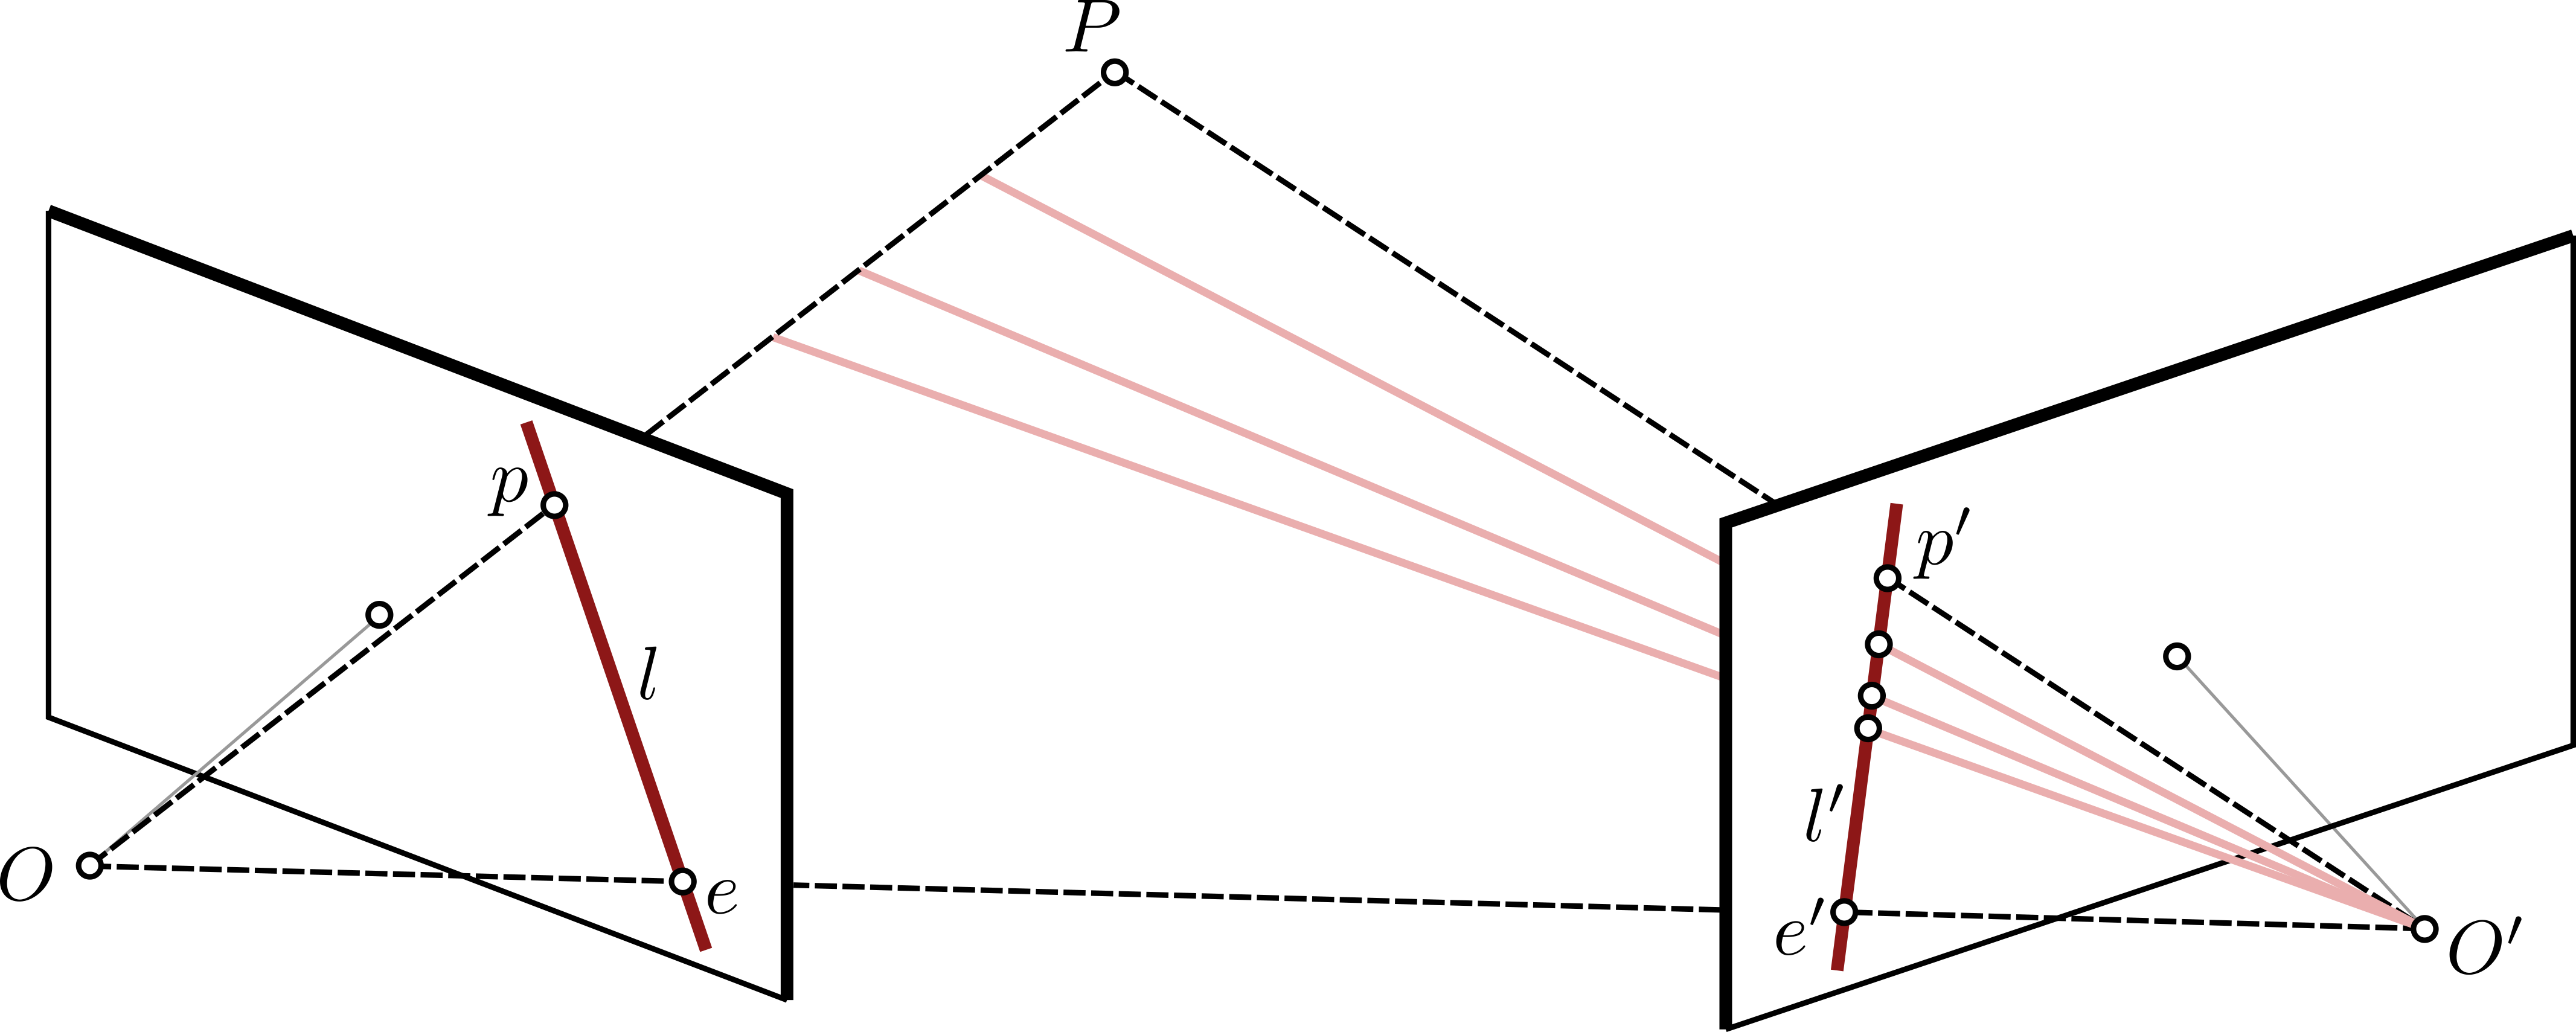
\includegraphics[width=.8\textwidth]{tex/figs/ch09_figs/stereo.png}
  \end{center}
  \caption{The point $P$ in the scene, the optical centers $O$ and $O'$ of the two cameras, and the two images $p$ and $p'$ of $P$ all lie in the same plane, referred to as the epipolar plane. The lines $l$ and $l'$ are the epipolar lines of the points $p$ and $p'$, respectively. Note that if the point $p$ is observed in one image, the corresponding point in the second image must lie on the epipolar line $l'$!}
  \label{fig:epi}
\end{figure}

Consider the images $p$ and $p'$ of a point $P$ observed by two cameras with optical centers $O$ and $O'$ (see Figure \ref{fig:epi}). These five points all belong to the \textit{epipolar plane} defined by the two intersecting rays $OP$ and $O'P$. 
In particular, the point $p$ lies on the line $l$ where the epipolar plane and the image plane intersect. The line $l$ is referred to as the \textit{epipolar line} associated with the point $p$, and it passes through the point $e$ (referred to as the \textit{epipole}).
Based on this geometry, if $p$ and $p'$ are images of the same point $P$, then $p$ must lie on the epipolar line $l$ and $p'$ must lie on the epipolar line $l'$. 

Therefore, when searching for correspondences between $p$ and $p'$ for a particular point $P$ in the scene it makes sense to restrict the search to the corresponding epipolar line. This is referred to as an \textit{epipolar constraint}, and greatly simplifies the correspondence problem by restricting the possible candidate points to a line rather than the entire image (i.e. a one dimensional search rather than a two dimensional search).
Mathematically, the epipolar constraints can be written as:
\begin{equation}
\overline{Op} \cdot [\overline{OO'} \times \overline{O'p'}] = 0, 
\end{equation}
since $\overline{Op}$, $\overline{O'p'}$, and $\overline{OO'}$ are coplanar. Assuming the world reference frame is co-located with camera 1 (with an origin at point $O$) this constraint can be written as:
\begin{equation} \label{eq:epiconst}
    p^\top  F p'=0,
\end{equation}
where $F$, referred to as the \textit{fundamental matrix}, has seven degrees of freedom and is singular. For a derivation of the epipolar constraint see Section 7.1 from Forsyth et al.\cite[]{ForsythPonce2011}. Additionally, the matrix $F$ is only dependent on the intrinsic camera parameters for each camera and the geometry that defines their relative positioning, and can be assumed to be constant. The expression for the fundamental matrix in terms of the camera intrinsic parameters is:
\begin{equation}
    F = K^{-\top}EK'^{-1}, \quad E = \begin{bmatrix}
    0 & -t_3 & t_2 \\
    t_3 & 0 & -t_1 \\
    -t_2 & t_1 & 0
    \end{bmatrix}R,
\end{equation}
where $K$ and $K'$ are the intrinsic parameter matrices for cameras 1 and 2 respectively, and $R$ and $t = [t_1, t_2, t_3]^\top $ are the rotation matrix and translation vector that map camera 2 frame coordinates into camera 1 frame coordinates.
Note that with the epipolar constraint defined by the fundamental matrix \eqref{eq:epiconst}, the epipolar lines $l$ and $l'$ can be expressed by $l = Fp'$ and $l' = F^\top p$. Additionally, it can be shown that $F^\top e = Fe' = 0$ where $e$ and $e'$ are the epipoles in the image frames of cameras 1 and 2, since by definition the translation vector $t$ is parallel to the coordinate vectors of the epipoles in the camera frames. This in turn guarantees that the fundamental matrix $F$ is singular.

If the parameters $K$, $K'$, $R$, and $t$ are not already known, the fundamental matrix $F$ can be determined in a manner similar to the intrinsic parameter matrix $K$ in the previous chapter. Suppose a number of corresponding points $p^h = [u, v, 1]^\top $ and $(p^h)'= [u',v',1]^\top $ are known and are expressed as homogeneous coordinates. Each pair of points has to satisfy the epipolar constraint \eqref{eq:epiconst}, which can be written as:
\begin{equation*}
\begin{bmatrix}
u & v & 1
\end{bmatrix} \begin{bmatrix}
F_{11} & F_{12} & F_{13} \\
F_{21} & F_{22} & F_{23} \\
F_{31} & F_{32} & F_{33}
\end{bmatrix} \begin{bmatrix}
u' \\ v' \\ 1
\end{bmatrix} = 0    
\end{equation*}
This expression can then be equivalently expressed by reparameterizing the matrix $F$ in vector form $f$ as:
\begin{equation}
\begin{bmatrix}
uu' & uv' & u & vu' & vv' & v & u' & v' & 1
\end{bmatrix}f = 0
\end{equation}
where $f = [F_{11}, \:F_{12} , \: F_{13}, \:F_{21}, \:F_{22}, \:F_{23}, \:F_{31}, \:F_{32}, \:F_{33}]^\top $. For $n$ known correspondences $(p,p')$ these constraints can be stacked to give:
\begin{equation}
    Wf = 0,
\end{equation}
where $W \in \R^{n \times 9}$.
Given $n \geq 8$ correspondences, an estimate $\tilde{F}$ of the fundamental matrix estimate is given by:
\begin{equation} \label{eq:fopt}
\begin{split}
\min_{f} \:\:& \lVert Wf \rVert^2, \\
\text{s.t.} \:\:& \lVert f \rVert^2 = 1.
\end{split}
\end{equation}
Note that the estimate $\tilde{F}$ computed by \eqref{eq:fopt} is not guaranteed to be singular. A second step is therefore taken to enforce this additional condition. In particular it is desirable to find the matrix $F$ that is closest to the estimate $\tilde{F}$ that has a rank of two:
\begin{equation}
\begin{split}
   \min_F \:\:& \lVert F-\tilde{F}\rVert^2, \\
\text{s.t.} \:\:& \text{det}(F) = 0,
\end{split}
\end{equation}
which can be accomplished by computing a singular value decomposition of the matrix $\tilde{F}$.

\subsubsection{Image Rectification}
Given a pair of stereo images, epipolar rectification is a transformation of each image plane such that all corresponding epipolar lines become colinear and parallel to one of the image axes, for convenience usually the horizontal axis. The resulting rectified images can be thought of as acquired by a new stereo camera obtained by rotating the original cameras about their optical centers. The great advantage of the epipolar rectification is the correspondence search becomes simpler and computationally less expensive because the search is done along the horizontal lines of the rectified images. The steps of the epipolar rectification algorithm are illustrated in Figure \ref{fig:rect}. Observe that after the rectification, all the epipolar lines in the left and right image are colinear and horizontal.
For an in-depth discussion on algorithms for image rectification see \cite{Fusiello2000}\cite{LoopZhang1999}.
\begin{figure}[ht]
  \begin{center}
	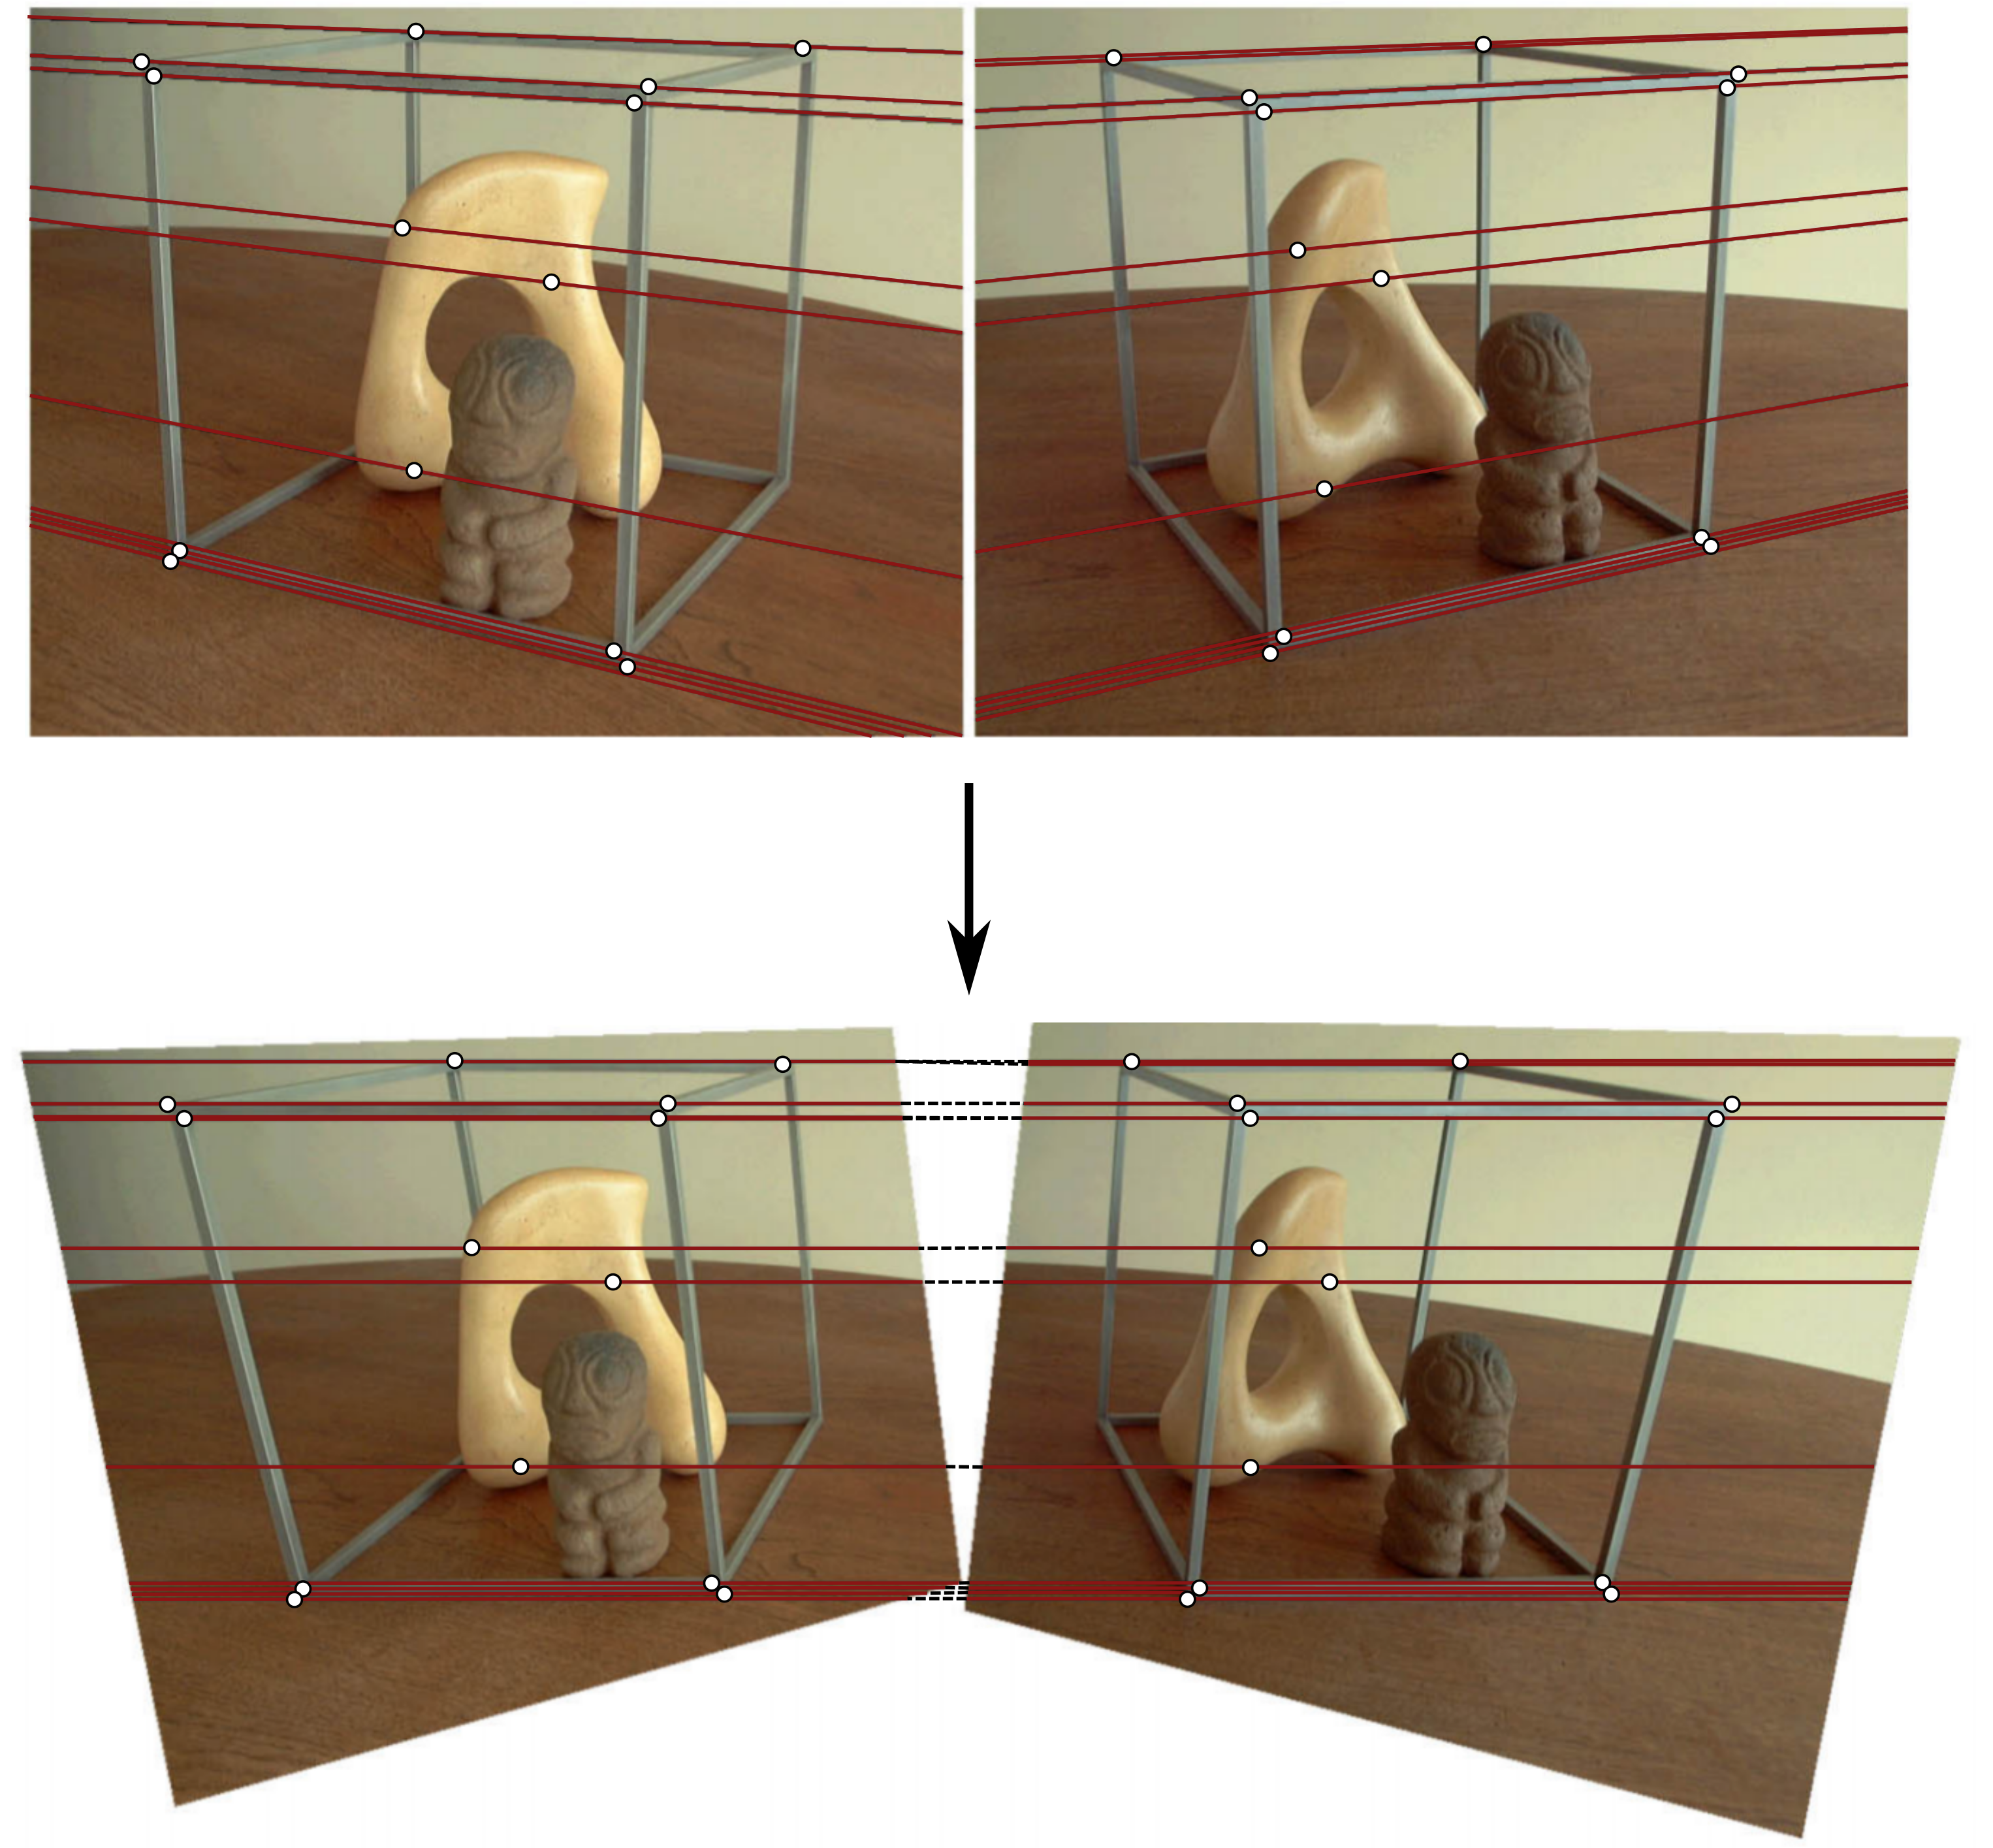
\includegraphics[width=0.7\textwidth]{tex/figs/ch09_figs/rectification.png}  \end{center}
  \caption{Epipolar rectification example from Loop et al. (1999).}
  \label{fig:rect}
\end{figure}

\subsubsection{Correspondence Problem}
Epipolar constraints and image rectification are commonly used in stereo vision to address the problem of correspondence, which is the problem of determining the pixels $p$ and $p'$ from two different cameras with different perspectives that correspond to the same scene feature $P$. While these concepts make finding correspondences easier, there are still several challenges that must be overcome. These include challenges related to feature occlusions, repetitive patterns, distortions, and others.

\subsubsection{Reconstruction Problem}

\begin{figure}[ht]
\centering
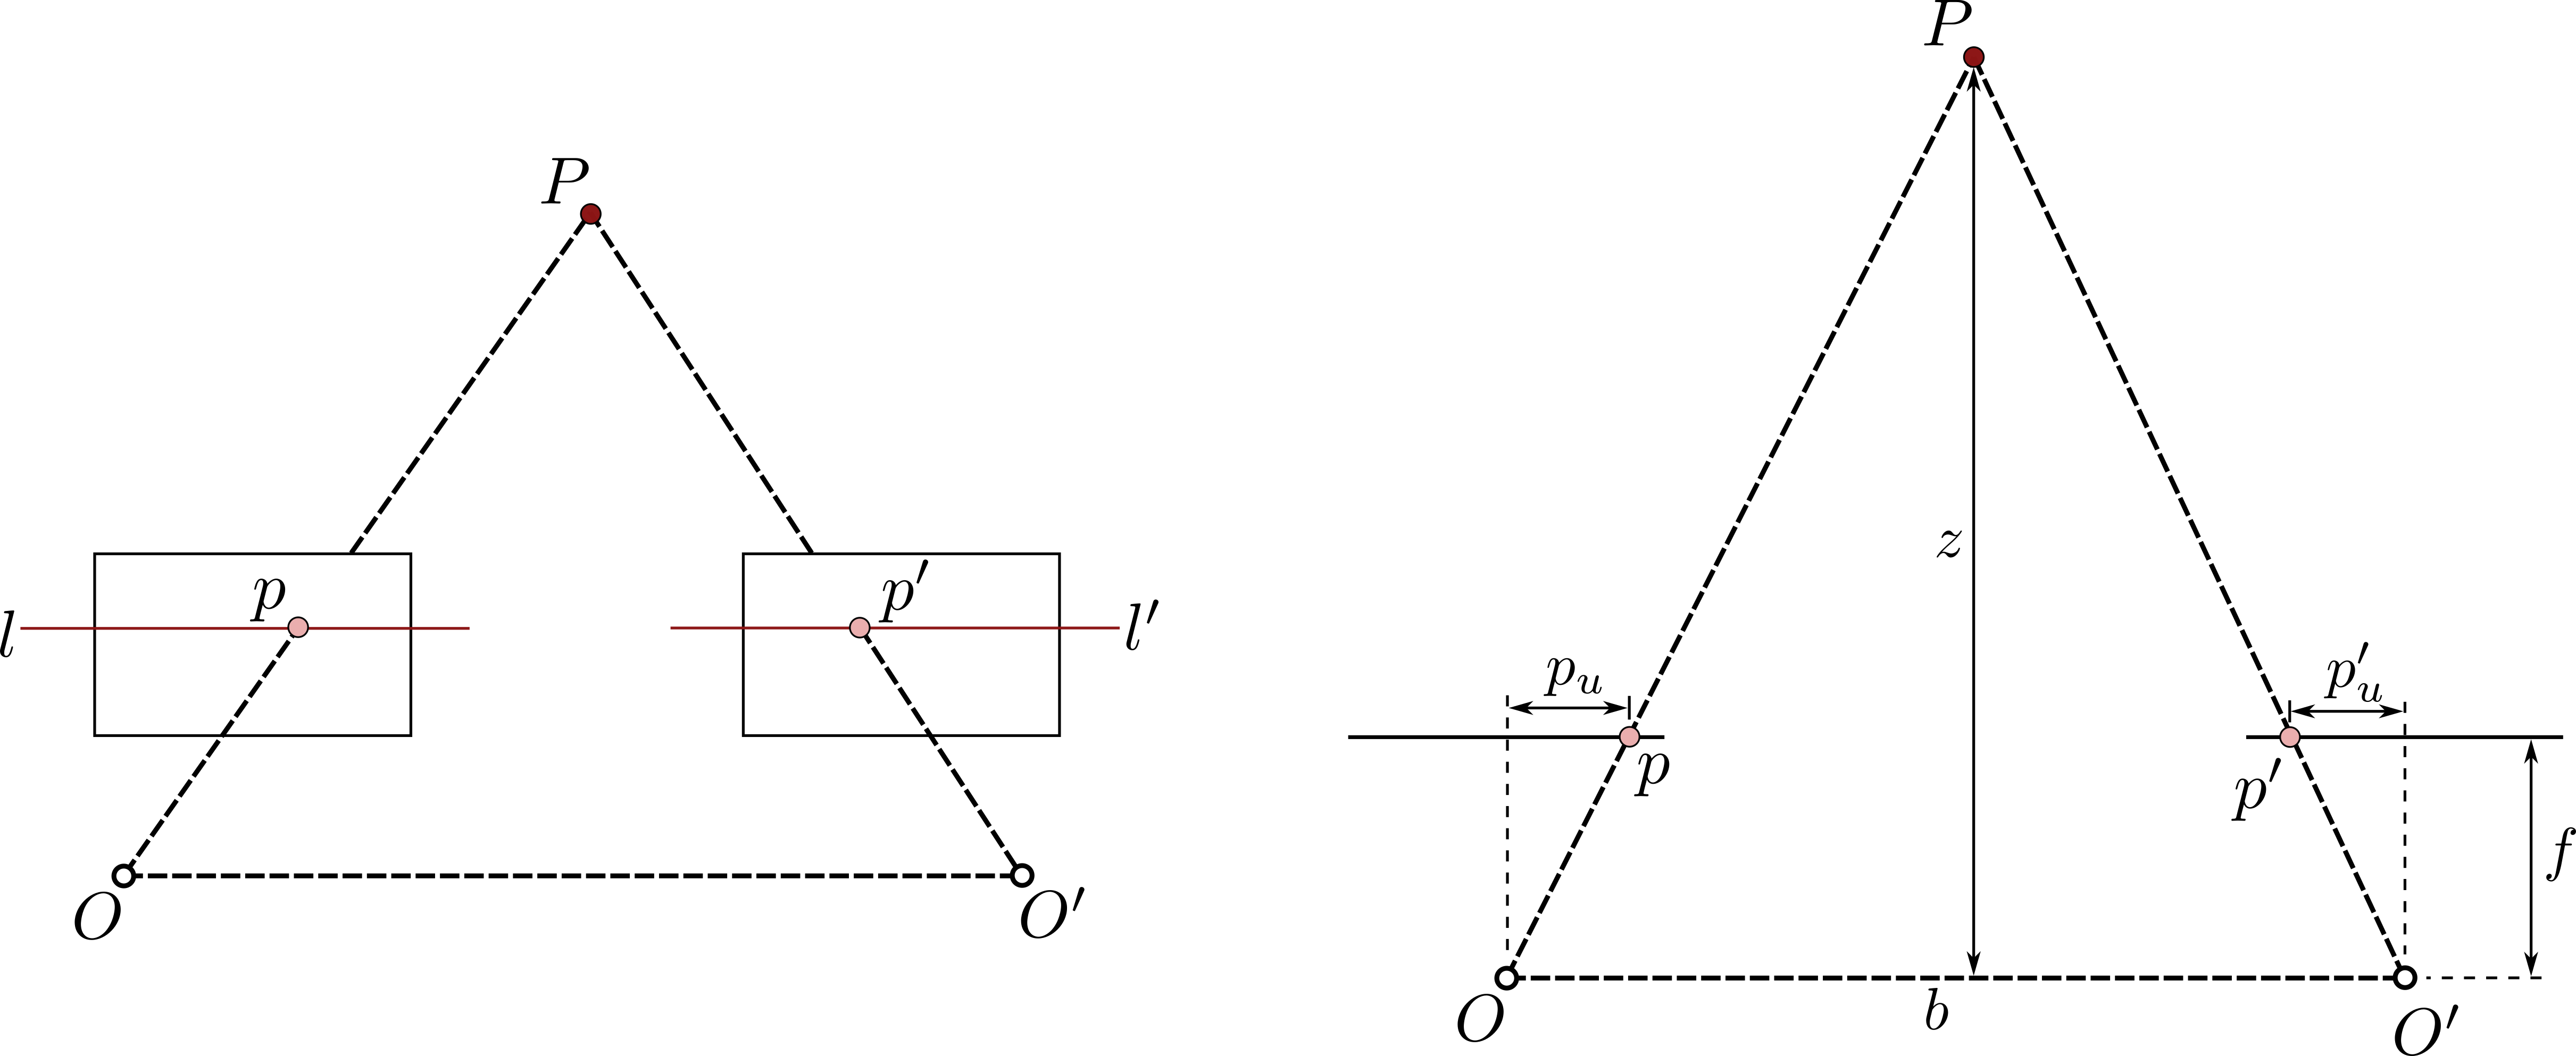
\includegraphics[width=0.9\textwidth]{tex/figs/ch09_figs/triangulation.png}
\caption{Triangulation with rectified images (horizontal view on the left, top-down view on the right).}
\label{fig:recttri}
\end{figure}
In a stereo vision setup, once a correspondence between the two images is identified it is possible to reconstruct the 3D scene point based on \textit{triangulation}. This process of triangulation has already been covered by the discussion on the epipolar geometry. However if the images have also be rectified such that the epipolar lines become parallel to the horizontal image axis the triangulation problem becomes simpler. This occurs, for example, when the two cameras have the same orientation, are placed with their optical axes parallel, and are separated by some distance $b$ called the \textit{baseline} (see Figure \ref{fig:recttri}).

In Figure \ref{fig:recttri}, a point $P$ on the object is described as being at coordinate $(x,y,z)$ with respect to the origin located in the left camera at point $O$. The horizontal pixel coordinate in the left and right image are denoted by $p_u$ and $p'_u$ respectively. Based on the geometry the depth of the point $P$ can be computed from the properties of similar triangles:
\begin{align}
  \frac{z}{b} &= \frac{z-f}{b-p_u+p'_u},
\end{align}
which can be algebraically simplified to:
\begin{equation}
    z = \frac{bf}{p_u-p'_u},
\end{equation}
where $f$ is the focal length. Generally a small baseline $b$ will lead to larger depth errors, but a large baseline $b$ may cause features to be visible from one camera but not the other. The difference in the image coordinates, $p_u-p'_u$, is referred to as \textit{disparity}. This is an important term in stereo vision, because it is only by measuring disparity that depth information can be recovered. The disparity can also be visually represented in a \textit{disparity map} (for example see Figure \ref{fig:disparity}), which is simply a map of the disparity values for each pixel in an image. The largest disparities occur from nearby objects (i.e. since disparity is inversely proportional to $z$).
\begin{figure}[ht]
\centering
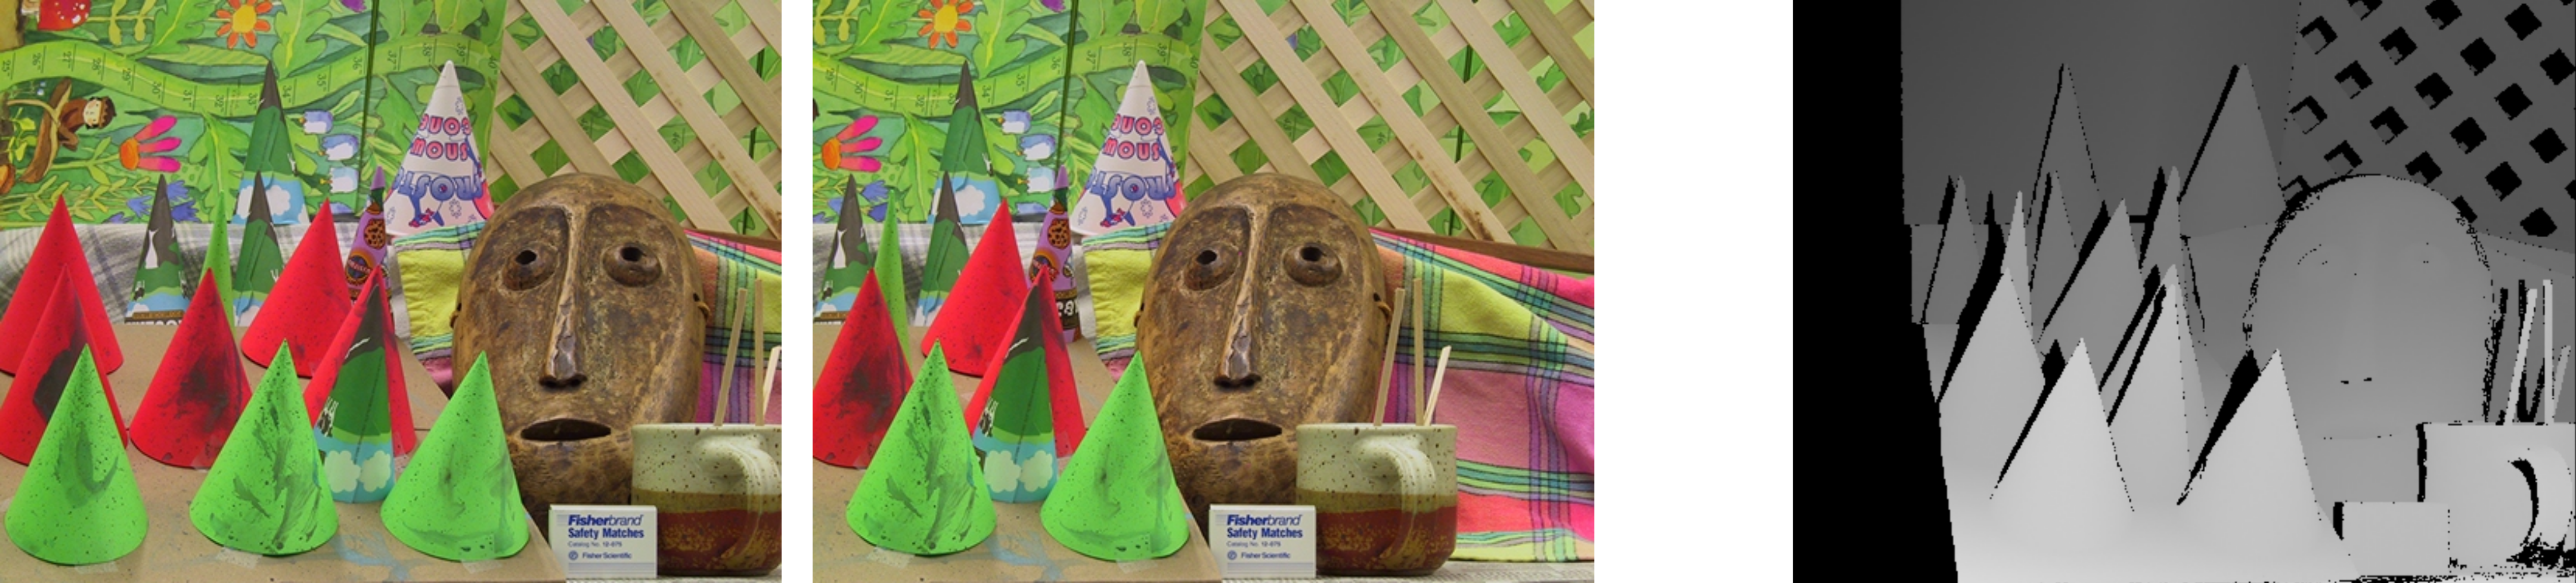
\includegraphics[width=0.95\textwidth]{tex/figs/ch09_figs/disparitymap.png}
\caption{Disparity map from a pair of stereo images. Notice that the lighter values of the disparity map represent larger disparity, and correspond to the point in the scene that are closer to the cameras. The black points represent points that were occluded from one of the images and therefore no correspondence could be made. Images from Scharstein et al. (2003) \nocite{ScharsteinSzeliski2003}.}
\label{fig:disparity}
\end{figure}

\subsection{Structure From Motion (SFM)}
The structure from motion (SFM) method uses a similar principle as stereo vision, but uses \textit{one} camera to capture multiple images from different perspectives while moving within the scene. In this case, the intrinsic camera parameter matrix $K$ will be constant, but the extrinsic parameters (i.e. the rotation matrix $R$ and relative position vector $t$) will be different for each image.
\begin{figure}[ht]
  \begin{center}
	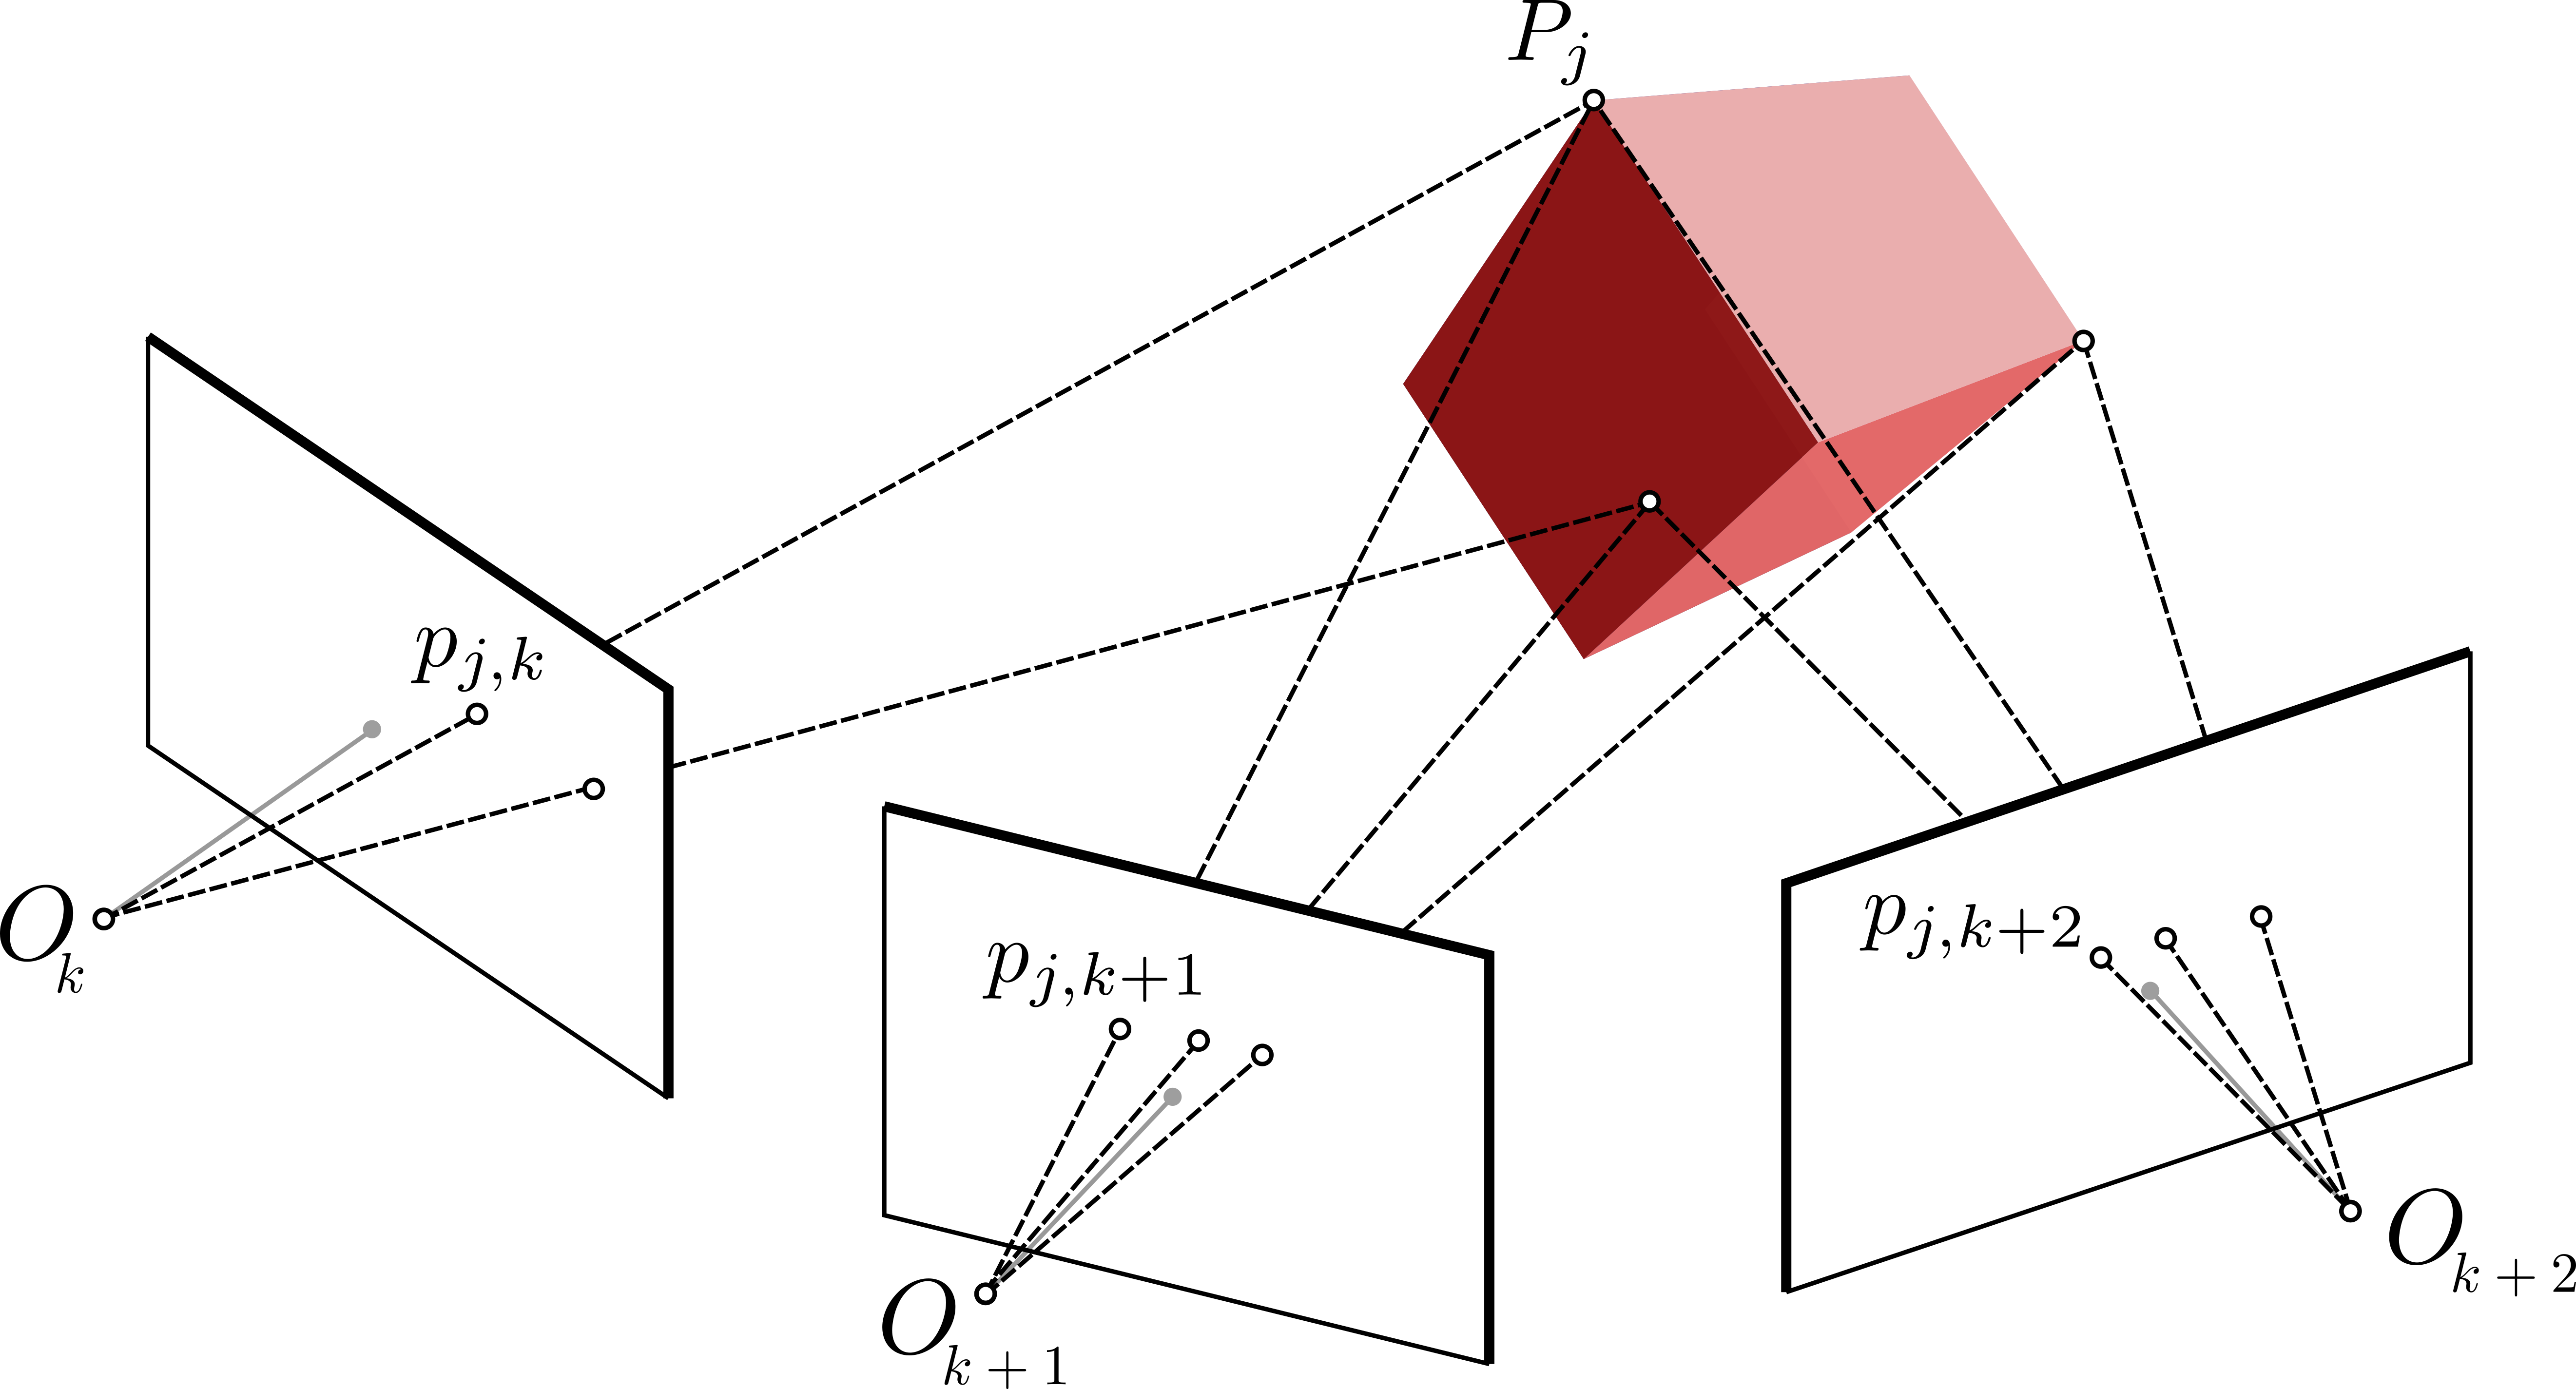
\includegraphics[width=0.75\textwidth]{tex/figs/ch09_figs/sfm.png}  \end{center}
  \caption{A depiction of the structure from motion (SFM) method. A single camera is used to take multiple images from different perspectives, which provides enough information to reconstruct the 3D scene.}
  \label{sfm}
\end{figure}
Consider a case where $m$ images of $n$ fixed 3D points are taken from different perspectives. This would involve $m$ homography matrices $M_k$ and $n$ 3D points $P_j$ that would need to be determined by leveraging the relationships:
\begin{equation*}
    p_{j,k}^h = M_k P^h_j, \quad j = 1,\dots,n, \quad k=1,\dots,m.
\end{equation*}

However, SFM also has some unique disadvantages, such as an ambiguity in the absolute scale of the scene that cannot be determined. For example a bigger object at a longer distance and a smaller object at a closer distance may yield the same projections.

One application of the SFM concept is known as \textit{visual odometry}. Visual odometry estimates the motion of a robot by using visual inputs (and possible additional information). This approach is commonly used in practice, for example by rovers on Mars, and is useful because it not only allows for 3D scene reconstruction but also to recover the motion of the camera.
